\documentclass[a5paper]{article}
\usepackage[a5paper, top=8mm, bottom=8mm, left=8mm, right=8mm]{geometry}

\usepackage{polyglossia}
\setdefaultlanguage[babelshorthands=true]{russian}

\usepackage{fontspec}
\setmainfont{FreeSerif}
\newfontfamily{\russianfonttt}[Scale=0.7]{DejaVuSansMono}

\usepackage[font=scriptsize]{caption}

\usepackage{amsmath}
\usepackage{amssymb,amsfonts,textcomp}
\usepackage{color}
\usepackage{array}
\usepackage{hhline}
\usepackage{cite}

\usepackage[hang,multiple]{footmisc}
\renewcommand{\footnotelayout}{\raggedright}

\PassOptionsToPackage{hyphens}{url}\usepackage[xetex,linktocpage=true,plainpages=false,pdfpagelabels=false]{hyperref}
\hypersetup{colorlinks=true, linkcolor=blue, citecolor=blue, filecolor=blue, urlcolor=blue, pdftitle=1, pdfauthor=, pdfsubject=, pdfkeywords=}

\newlength\Colsep
\setlength\Colsep{10pt}

\usepackage{tabu}

\usepackage{graphicx}
\usepackage{indentfirst}
\usepackage{multirow}
\usepackage{subfig}
\usepackage{footnote}
\usepackage{minted}
\usepackage{xcolor}

\tabulinesep=1.2mm

\newcommand{\attribution}[1] {
\vspace{-5mm}\begin{flushright}\begin{scriptsize}\textcolor{gray}{\textcopyright\, #1}\end{scriptsize}\end{flushright}
}

\sloppy
\pagestyle{plain}

\title{Основы сетевой безопасности}
\author{Юрий Литвинов\\\small{y.litvinov@spbu.ru}}

\date{19.10.2021}

\begin{document}

\maketitle
\thispagestyle{empty}

\section{Введение}

Вообще, темасетевой безопасности заслуживает отдельного курса, но кое-какие вещи, типа тех же сертификатов, необходимы любому программисту в повседневной работе, так что обойти их обсуждение хотя бы кратко не получится. В современном мире почти все сервисы требуют аутентификации, авторизации и обеспечения безопасности. Причём, обратите внимание, что аутентификацию и авторизацию часто путают, это разные вещи:

\begin{itemize}
    \item \textit{аутентификация} --- это установление личности (точнее, идентичности) участника взаимодействия; личность нам не важна, нам важно знать, что это тот пользователь, о котором мы думаем, или хотя бы пользователь из той группы пользователей с одинаковыми правами, за которого себя выдаёт; аутентификация часто взаимна --- сервер не доверяет клиенту, но и клиент не может быть уверен в том, что сервер не подделан злоумышленником;
    \item \textit{авторизация} --- это установление прав на выполнение операции, когда аутентификация уже выполнена. Вы можете быть вполне легитимным пользователем GMail, но это не значит, что вы имеете право просматривать мою почту; или вы можете иметь доступ только на чтение к какому-то документу.
\end{itemize}

\textit{Шифрование} --- это обеспечение конфиденциальности передаваемой информации. Но для информационной безопасности важна не только конфиденциальность, но и:

\begin{itemize}
    \item \textit{целостность} --- что злоумышлениик ничего не поменял в сообщении; даже не имея возможности его прочитать, он может нанести ущерб, внеся изменения, если они не будут замечены получателем;
    \item \textit{актуальность} --- что злоумышленник не проиграл просто старое сообщение; ведь не надо ни дешифровать, ни изменять как-то ваше сообщение об оплате мобильной связи, чтобы лишить вас всех денег, если протокол оплаты не обеспечивает свойство актуальности.
\end{itemize} 

\section{Шифрование}

Классическая схема шифрования предполагает передачу конфиденциальных данных по каналу, который может прослушивать злоумышленник (так называемая схема с пассивным злоумышленником) или злоумышленник может модифицировать сообщения в канале (схема с активным злоумышленником):

\begin{center}
    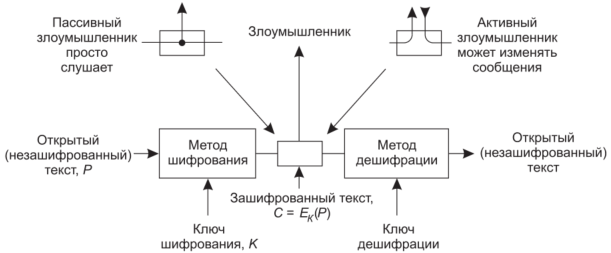
\includegraphics[width=0.8\textwidth]{cryptography.png}
    \attribution{Э. Таненбаум}
\end{center}

Незашифрованный текст называется в англоязычной литературе Plaintext и поэтому обозначается P. Зашифрованный текст называется Ciphertext и обозначается C. Алгоритм шифрования (Encryption, E) использует параметр K (Key) --- ключ шифрования, по которому преобразует открытый текст в зашифрованный: $C = E_K(P)$. Алгоритм дешифрования (Decryption, D) использует ключ дешифрации (тот же, или отличающийся от K), чтобы построить обратно открытый текст по его зашифрованному варианту.

\noindent\begin{minipage}{\textwidth}
    \begin{minipage}[c][4cm][c]{\dimexpr0.7\textwidth-0.7\Colsep\relax}
        В криптографии традиционно считается, что сам алгоритм шифрования известен, неизвестен только ключ. Связано это с тем, что хороший алгоритм шифрования разработать сложно (это занимает годы) и если его взломают, придётся менять и сам алгоритм, и его программные и аппаратные реализации. Это сложно и дорого. Если взломают ключ, достаточно выбрать другой. Более того, современные алгоритмы заранее меняют ключи раз в несколько секунд, чтобы осложнить злоумышленнику криптоанализ.
    \end{minipage}\hfill
    \begin{minipage}[c][4cm][c]{\dimexpr0.3\textwidth-0.3\Colsep\relax}
        
\includegraphics[width=0.7\textwidth]{youAreBeingWatched.png}
    \end{minipage}%
\end{minipage}

Ещё стоит помнить, что алгоритмы шифрования --- это суровая алгебра, теория чисел и теория вероятностей. Если вы думаете, что криптосхема <<кручу-верчу, запутать хочу>> или последовательное применение двадцати разных алгоритмов шифрования повысит криптостойкость вашего метода шифрации, вас могут ждать неприятные сюрпризы (вплоть до того, что криптостойкость внезапно понизится). Повысить криптостойкость можно увеличением размера ключа, но во многих странах существуют законодательные ограничения на длину ключа в гражданских шифрах. Связано это не с тем, что тоталитарный режим хочет следить за всеми своими гражданами (хотя хочет, конечно), а с тем, что при крайней необходимости (например, постановлении суда) и затратой больших вычислительных ресурсов (например, суперкомпьютера ВМК МГУ) сообщение всё-таки можно было бы расшифровать. Военные шифры имеют такую длину ключа, что дешифровка сообщений по крайней мере грубой силой на всех нынешних и будущих вычислительных ресурсах планеты даже по оптимистичным оценкам займёт время большее, чем нужно Солнцу, чтобы исчерпать запасы водорода и погаснуть.

Подавляющее большинство интернет-трафика шифруется шифрами с симметричным ключом (то есть ключом, одинаковым для шифровки и дешифровки), потому что они работают очень быстро. Обратите внимание, речь идёт не о шифровании секретных донесений шпионов или банковских переводов, а о шифровании вообще всего трафика --- любой веб-страницы, скачиваемых файлов и даже фильмов, которые вы смотрите через стриминговые сервисы (казалось бы, что секретного в фильме, который и так может посмотреть любой желающий, но если посторонние узнают тот факт, что вы его смотрите --- это privacy violation). Поэтому современные процессоры имеют даже аппаратную поддержку симметричных шифров. 

Однако аутентификация и выбор ключа для последующей симметричной передачи выполняются с помощью асимметричных шифров --- шифров, которые используют разные ключи на стороне отправителя и получателя. Асимметричные шифры хороши тем, что могут использовать открытые ключи, которые позволяют отправителю и получателю вообще не обмениваться никакими секретами. 

Как это возможно? Алгоритм шифрования делится на две части, $D$ и $E$ так, что $D(E(P)) = P$ (этим свойством обладает большинство криптосхем). В отличие от симметричного шифрования, протоколы с открытым ключом используют разные ключи от $D$ и $E$ и обладают тем свойством, что ключ от $D$ очень сложно получить, зная только ключ от $E$ (например, для этого надо найти простые сомножители огромного числа или дискретный логарифм по заданному модулю). Ключ от $D$ держится в секрете, ключ от $E$ выкладывается в открытый доступ.

Теперь, положим, Боб хочет послать Алисе сообщение\footnote{Участники взаимодействия по традиции называются Алиса и Боб (А и Б)}. Боб берёт открытый ключ Алисы $E_A$, шифрует им сообщение $P$ и отправляет Алисе. Алиса легко дешифрует сообщение, вычисляя $D_A(E_A(P))$. Злоумышленник не может прочитать сообщение, поскольку не знает $D_A$ и не может его получить. Если Алиса хочет послать сообщение Бобу, она берёт открытый ключ Боба и делает то же, что и Боб. Популярных алгоритмов, построенных по такой схеме, сразу несколько: RSA (основанный на разложении на простые множители), ElGamal (основанный на дискретных логарифмах), эллиптические шифры (основанные вообще на алгебре точек на эллиптических кривых). Все они где-то на самом деле используются.

\subsection{Цифровые подписи}

Шифровать всё сообщение асимметричным шифром слишком трудоёмко, а иногда нам не нужно обеспечить конфиденциальность сообщения, достаточно лишь гарантировать, что сообщение было послано тем, кем мы думаем, что они было послано, и не было изменено в процессе передачи. Пример ситуации, когда это нужно --- библиотеки .NET, выкладываемые в NuGet или распространяемые как часть приложений. Было бы не очень здорово, если бы вместо NUnit в NuGet выложили библиотеку, которая собирает данные банковских карточек с любого компьютера, на котором запущена. Для того, чтобы так не было, используются цифровые подписи:

\begin{center}
    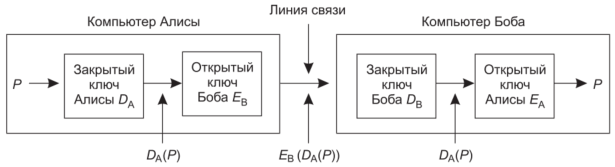
\includegraphics[width=0.8\textwidth]{signature.png}
    \attribution{Э. Таненбаум}
\end{center}

Тут Алиса хочет послать сообщение Бобу так, чтобы Боб мог убедиться, что сообщение действительно послала Алиса, и был бы уверен, что Алиса потом не будет отпираться, что послала сообщение. Алиса сначала шифроует сообщение своим закрытым ключом $D_A$, а затем, как обычно, шифрует то, что получилось, открытым ключом Боба $E_B$. Боб, получив такое сообщение, сначала прменяет свой закрытый ключ, затем открытый ключ Алисы (он его знает, потому что Алиса заранее его опубликовала), получая тем самым исходное сообщение. Он точно знает, что автором была Алиса, потому что если бы автором был кто-то ещё, он бы не знал ключа $D_A$ и при применении $E_A$ получилась бы каша. 

Ну а теперь, собственно, как не шифровать всё сообщение. Давайте сначала по нешифрованному сообщению посчитаем дайджест (Message Digest) --- хорошую хеш-функцию от сообщения, которая обладает таким свойством, что вычисляется по сообщению однозначно, но даже малое изменение сообщения (буквально в одном бите) до неузнаваемости меняет хеш-значение. При этом хеш-функция должна считаться быстро, и по данному хеш-значению должно быть невозможно получить исходное сообщение никак кроме как перебором (что с учётом того, что хеш-функция неизбежно теряет информацию, довольно безнадёжно, перебор даст лишь пару миллионов подходящих сообщений, которые даже похожи на правду). 

Дальше берём посчитанное хеш-значение и подписываем его описанным выше способом только его. Хеш-значение обычно небольшое (например, 20 байт), так что это можно сделать быстро. Адресату шлётся сообщение открытым текстом (например, библиотека .NET) и подписанный хеш (та самая цифровая подпись). Адресат по открытому сообщению сам считает хеш и применяет открытый клю автора к подписанному хешу, сличая то, что получилось. Если хеши одинаковые, то либо сообщение правда было отправлено кем надо и не менялось, либо злоумышленнику удалось подобрать такое сообщение, которое даёт точно то же хеш-значение, что и исходное, и при этом ещё и имеет смысл (что для достаточно хороших хеш-функций статистически маловероятно, настолько, что этим можно пренебречь).

Распространённые криптографические хеш-функции --- это MD5 (старая и уязвимая хеш-функция, коллизии подбираются атакой дней рождения за вполне конечное время), семейство функций SHA (SHA-1, SHA-2, SHA-3). SHA-1 тоже научились ломать, хоть это вычислительно гораздо сложнее, чем MD5, так что для практических цифровых подписей используются более криптостойкие SHA-2 и SHA-3 (SHA-3 относительно новая и не успела стать популярной).

\subsection{Сертификаты}

Окей, теперь мы зная открытый ключ нашего собеседника без проблем проверим, что он тот, за кого он себя выдаёт, но как мы узнаем, что у нас на самом деле правильный открытый ключ нашего собеседника? Понятно, что мы могли бы получить его на флешке, но если бы для того, чтобы ходить во вконтактик, всем пришлось бы ехать за ключом на Невский, никто бы вконтактиком не пользовался. Мы могли бы скачать открытый ключ со страницы нашего собеседника (например, того же vk.com), но злоумышленник довольно без проблем (до сих пор, несмотря на внедрение DNSSec!) может перехватить ваш запрос к странице и отправить вас на свою страницу, которая будет выглядеть точно так же, как vk.com, но содержать открытый ключ злоумышленника. А дальше --- атака Man In The Middle:

\begin{center}
    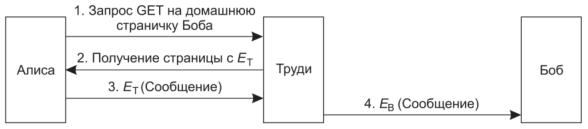
\includegraphics[width=0.8\textwidth]{manInTheMiddle.png}
    \attribution{Э. Таненбаум}
\end{center}

Чтобы такой беды не было, давайте, мм, подписывать открытые ключи. Боб, публикуя свой открытый ключ, получает у кого-то, кому доверяет и Алиса, и Боб, сообщение, что это правда открытый ключ Боба, подписанное этим кем-то, кому все доверяют. Теперь Алиса, получив открытый ключ Боба, может проверить подпись в этом сообщении и убедиться, что это правда ключ Боба. Но что будет, если Труди (от английского inTruder) взломает страницу того, кому все доверяют, и подсунет свой ключ вместо его ключа, заставив тем самым Боба подписать своё ключ фальшивой подписью, которую Труди без проблем сможет подделать во время атаки Man In The Middle? Хм, давайте подпишем и этот ключ, и тот ключ, которым мы подписали этот ключ, и т.д. по цепочки, до Ключа, Которому Точно Все Доверяют. Такой ключ (точнее, несколько десятков их) могут быть вшиты в поставку операционной системы, браузера и т.п., так что при получении сообщения Алиса может проверить подписи по цепочке до ключа, который она получила от, например, Microsoft, и знает, что у злоумышленника вряд ли хватит денег, чтобы убедить Microsoft подсунуть фальшивый ключ.

Именно так работают \textit{сертификаты}. Сертификат --- это то самое сообщение, подтверждающее идентичность ключа (что-то вида <<предъявитель сего действительно является Иваном Ивановым, владельцем домена example.com>>), подписанное Certificate Authority (CA). Сертификаты имеют фиксированный формат, определяемый стандартом X.509, довольно ужасным, но по сути сводящемся к набору пар <<ключ-значение>>, хранящих информацию о владельце сертификата. Сертификаты бывают разные, от самых простых, что предъявитель сего владеет таким-то доменом, даже без указания имени хозяина, до сертификатов, выдаваемых интернет-магазинам сертификационными центрами, которые подтверждают, что владелец сертификата действительно может заниматься интернет-торговлей, не обманет и достаточно финансово устойчив, чтобы не обанкротиться, пока доставляет вашу покупку.  Понятно, что такие сертификаты стоят денег, и иногда немалых (и выдаются только на время, кстати).

CA верхнего уровня подписывают сертификаты CA уровнем ниже, чтобы те могли подписывать уже сертификаты конечных пользователей. Таким образом, получается цепочка сертификатов от конкретного пользователя до корневого CA, сертификаты которого общеизвестны и им все доверяют. При передаче сообщения передают всю цепочку сертификатов сразу, чтобы для проверки подписей вообще не требовалось выполнять сетевые запросы, благо сертификаты очень небольшие. Получатель может проследить, что все сертификаты в цепочке подписаны друг другом и цепочка заканчивается на сертификате, которому получатель точно доверяет, потому что, например, получил его десять лет назад вместе с новым компьютером. Такие доверенные сертификаты называются корневыми (root certificates) и хранятся в специальном хранилище в ОС любого компьютера.

Поскольку настоящие сертификаты как минимум требуют что-то подтвердить, а как максимум стоят как недорогая иномарка, для отладки сетевых приложений используют \textit{самоподписанные} сертификаты. Это сертификат, который разработчик может сгенерировать сам, ему, понятное дело, никто не доверяет, потому что невозможно отследить его цепочку доверия до корневого сертификата, но разработчик может сам добавить такой сертификат в список доверенных. Тогда все приложения, пользующиеся системными сервисами проверки сертификатов, будут вынуждены ему доверять. Именно так работает Fiddler, когда дешифрует HTTPS-трафик, кстати. Visual Studio, кстати, умеет генерировать самоподписанные сертификаты: \url{https://docs.microsoft.com/en-us/windows/msix/package/create-certificate-package-signing}, но чаще это делают через инструменты библиотеки OpenSSL. 

А вот бесплатное CA, выдающее сертификаты, доказывающие владение доменом: \url{https://letsencrypt.org/}. Ему более-менее все современные браузеры доверяют, так что там можно получить вполне доверенный сертификат, которым можно защищать HTTPS-соединение. Код им подписывать не получится, но по крайней мере, шифровать соединение с сайтом вполне можно (а это необходимо для любого нормального протокола аутентификации). Так что в современном мире неиспользование HTTPS по причине дороговизны сертификата больше не является валидным.

\subsection{HTTPS}

Собственно, сертификаты используются очень много где, но в контексте сетевых приложений они наиболее важны для установки HTTPS-соединения. HTTPS --- это обычный протокол HTTP, использующий Secure Sockets Layer, или SSL, в качестве протокола уровня представления. Установление соединения по HTTPS включает в себя аутентификацию сервера на клиенте как раз через цепочку сертификатов. Клиент не должен доказывать свою идентичность серверу (об этом потом позаботится аутентификация, уже когда соединение будет установлено), но если сервер не сможет убедить клиента, что он правда тот, на который клиент пытается зайти (в смысле доменного имени), соединение даже установлено не будет.

Вот так примерно устроено установление соединения по HTTPS:

\begin{center}
    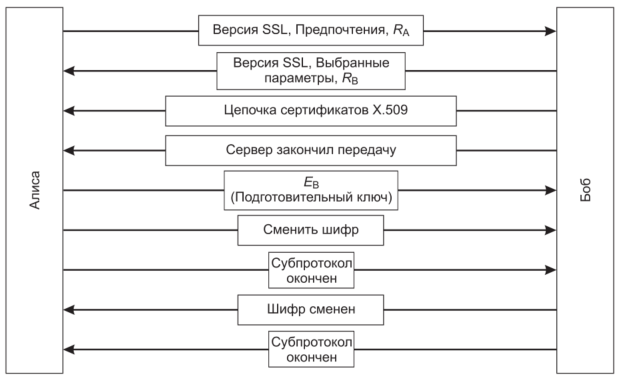
\includegraphics[width=0.8\textwidth]{ssl.png}
    \attribution{Э. Таненбаум}
\end{center}

Сначала Алиса и Боб договариваются о версии SSL и обмениваются одноразовыми ключами (\textit{nonce}, Number used once, просто случайные числа для предотвращения атаки повтором), затем Боб отправляет свою цепочку сертификатов, чтобы доказать, что он правда Боб, затем Алиса шифрует открытым ключом Боба подготовительный ключ для симметричного шифрования (который тоже выбирает случайно, используя nonce-ы), Боб, зная свой закрытый ключ и оба nonce-а, расшифровывает симметричный ключ, подтверждает получение Алисе и переходит на симметричный шифр с этим ключом. Ненадолго, впрочем, HTTPS предполагает частую смену симметричного ключа во избежание статистических атак.

\subsection{OAuth 2}

Последнее, с чем остальнос разобраться --- это с авторизацией. Хорошо, Алиса и Боб смогли подтвердить идентичность друг друга, но Алиса хочет зайти на файловое хранилище и скачать оттуда файл, Боб должен проверить, что она имеет на это право. Боб мог бы сам владеть и файловым хранилищем, и держать у себя таблицу, в которой написано, что Алиса имеет право делать, а что нет, и это бы даже хорошо работало, если бы Алиса только для этого и пользовалась интернетом. Но подумаем об обычном пользователе, который зареган на тысяче ресурсов. Если к каждому надо придумывать свой логин и пароль, можно сойти с ума. Если каждый ресурс знает логин и пароль пользователя, то если взломают хоть один, взломают и все остальные.

Поэтому появился протокол OAuth (тут речь пойдёт про OAuth 2, используемый ныне). Этот протокол позволяет разрешить пользование ресурсом, не раскрывая хозяину ресурса логин и пароль пользователя. Например, можно войти на сторонний ресурс по аккаунту в Google или аккаунту в VK, не сообщая при этом ресурсу никакой ценной информации о себе, не говоря уж о логине и пароле. Так можно помнить только пароль от Google и ходить на все остальные сайты, умеющие в OAuth, по нему. Светлая цель разработки такого протокола была вообще в том, чтобы был некий глобальный сервис аутентификации, которому все доверяют, и который бы позволял проверить идентичность пользователя и дать доступ ко всем остальным сайтам интернетов, но, во-первых, с <<которому все доверяют>> возникли проблемы, во-вторых, когда это человечество о чём-то хорошем договорилось.

Работает протокол примерно как на картинке из стандарта (RFC 6749):

\begin{center}
    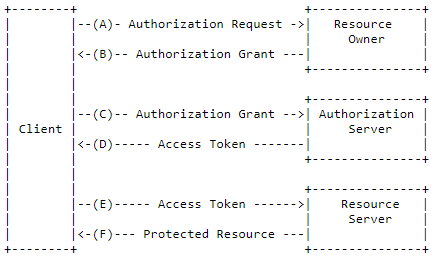
\includegraphics[width=0.6\textwidth]{oauth.png}
    \attribution{RFC 6749}
\end{center}

Client --- это приложение, которое хочет работать с каким-то ресурсом (например, браузерный клиент гуглодиска). Resource Owner --- это пользователь (человек), который может разрешить или не разрешить клиенту доступ к ресурсу. Authorization Server --- это то место, где разрешение на доступ к ресурсу можно обменять на Access Token, если Resource Owner реально имеет право на доступ к ресурсу. Дальше мы можем с этим Access Token-ом пойти на ресурсный сервер и предъявить уже Access Token, чтобы пользоваться ресурсом, не авторизуясь на нём ещё раз. Аутентификация и авторизация проводится только один раз, на Authorization Server-е, выдаваемый им токен устроен так, что Resource Server может легко проверить его валидность и то, что клиент действительно имеет право выполнять запрашиваемую операцию (очередное применение криптографических хешей, кстати).

Чаще всего протокол OAuth 2 используется в режиме Authorization Code, когда клиент не запрашивает у владельца ресурса авторизацию напрямую, а перенаправляет его на Authorization Server, где владелец аутентифицируется и авторизуется. При этом логин/пароль пользователя видит только Authorization Server, даже клиент не имеет к ним доступа. Authorization Server затем отвечает клиенту, отправляя ему Access Token (для чего используется некая магия с URL-ами). При этом Access Token имеет свойство протухать через некоторое небольшое время (чтобы если злоумышленник перехватит Access Token, он с меньшей вероятностью мог воспользоваться ресурсом), поэтому клиенту также обычно выдаётся Refresh Token --- токен, который можно обменять на новый Access Token, когда старый протухнет. Refresh Token живёт подольше (обычно от нескольких дней до пары месяцев) и его можно продлять, так что если пользователь часто пользуется ресурсом (например, ходит во вконтакт каждый день), ему вообще не надо авторизовываться. Refresh Token передаётся по сети довольно редко, так что несмотря на то, что он важнее, вероятность, что его перехватят, меньше. Напомним, что всё происходит по HTTPS, так что чтобы получить хоть один токен, сначала надо взломать относительно неломаемый протокол. А если его всё-таки взломают, Refresh Token часто можно вручную отозвать.

Так устроена большая часть существующих механизмов авторизации для веб-сайтов и веб-сервисов, поэтому с OAuth неплохо бы разобраться и хотя бы раз попробовать.

\end{document}
